% 隔離テスト用ドライバ: 01-04 のみを単独ビルド（共有 main.tex には影響しない）
\documentclass[11pt,aspectratio=43,dvipsnames]{beamer}
\usepackage{luatexja}
\usepackage[match]{luatexja-fontspec}
\setmainjfont{HaranoAjiGothic}
\setsansjfont{HaranoAjiGothic}
\renewcommand{\kanjifamilydefault}{\gtdefault}
\usepackage{amsmath, amssymb}
\usepackage[version=4]{mhchem}
\usepackage{booktabs}
\usepackage{multirow}
\usepackage{colortbl}
\usepackage{graphicx}
\graphicspath{{figures/}}
\usepackage{pgfplots}
\pgfplotsset{compat=1.18}
% =====================================================================
%  seminar テーマ定義（既存 Marp デザインの Beamer 再現）
%  ・濃青の恒常ヘッダーバー（セクション名＋ページ番号）
%  ・専用表紙（アクセントライン＋グラデ背景）
%  ・本文は白地・濃青見出し
%  main.tex から \input する（パッケージではなく生プリアンブル）
% =====================================================================

% ---- ベース：装飾の少ないテーマから組む -----------------------------
\usetheme{default}
\usefonttheme{professionalfonts}
\setbeamertemplate{navigation symbols}{}   % ナビゲーション記号を消す

% ---- TikZ（ヘッダー・表紙・矢印などで使用）-------------------------
\usepackage{tikz}
\usetikzlibrary{arrows.meta, positioning, calc, shapes.geometric, fit, patterns}

% ---- 配色（ルール準拠）---------------------------------------------
\definecolor{HeaderBlue}{HTML}{0f5a7a}   % ヘッダー・見出しの濃青
\definecolor{DateGray}{HTML}{334b5e}     % 表紙の日付グレー
\definecolor{TitleBG}{HTML}{edf5fb}      % 表紙グラデの薄青

% コンテンツ用パレット（図・ハイライト・矢印で共通利用）
\definecolor{ArrowBlue}{HTML}{1F6FC4}    % 矢印・強調の青
\definecolor{HiPink}{HTML}{F4B6BE}       % ハイライト見出し（暖色）
\definecolor{HiBlue}{HTML}{C7DCEF}       % ハイライト見出し（寒色）
\definecolor{IpaBlue}{HTML}{1F5FC4}      % グラフ系列1（青）
\definecolor{DipeOrange}{HTML}{E8821E}   % グラフ系列2（橙）
\definecolor{SpRed}{HTML}{C0392B}        % 反応式：プロピレン強調の赤
\definecolor{SpBlue}{HTML}{1F6FC4}       % 反応式：エテン・エタン・CH0.5 の青

% 帯（ヘッダーバー）のパート別配色（寒色グラデ）。本文枠線は HeaderBlue のまま。
%  1-4 導入・全体像／5-9 反応・反応器／10-13 分離／14-17 最適化・経済・結言
\definecolor{barA}{HTML}{0F5A7A}   % 1-4  青緑
\definecolor{barB}{HTML}{1D6E6E}   % 5-9  シアン寄り
\definecolor{barC}{HTML}{2E4C8A}   % 10-13 青
\definecolor{barD}{HTML}{4A3C84}   % 14-17 紫

\setbeamercolor{normal text}{fg=black, bg=white}
\setbeamercolor{frametitle}{fg=HeaderBlue, bg=white}
\setbeamercolor{itemize item}{fg=HeaderBlue}
\setbeamercolor{itemize subitem}{fg=HeaderBlue}
\setbeamercolor{block title}{fg=white, bg=HeaderBlue}
\setbeamercolor{block body}{fg=black, bg=TitleBG}
\setbeamercolor{alerted text}{fg=HeaderBlue}

% ---- フォントサイズ（Marp px をおおよそ pt に対応）------------------
\setbeamerfont{frametitle}{size=\large, series=\bfseries}   % スライド見出し ~44px

% ---- 恒常ヘッダーバー（headline）-----------------------------------
%  左：セクション名（無ければロゴ枠）／右：ページ番号
\newcommand{\HeaderLogo}{}   % ロゴを入れるなら \renewcommand で画像指定
% 本線の総枚数（分母）。appendix に入ると分子がこれを超え、本線/付録を見分けられる。
\newcommand{\MainTotal}{17}
% パート別に帯色を選ぶ：1-4=barA／5-9=barB／10-13=barC／14-17=barD。
% スライド4の独自帯（CC・GCC）など headline を上書きする箇所でも呼べるよう独立コマンド化。
% 併せて本文アクセント色 HeaderBlue 自体をそのパート色へ再定義し、各スライドの
% 図・枠線・矢印・ボックス（HeaderBlue 参照）をパート色に連動させる（\colorlet は大域的）。
% headline はフレーム本文より前に組まれるため、ここでの再定義が本文に効く。
\newcommand{\SetBarColor}{%
  \ifnum\insertframenumber<5\setbeamercolor{headerbar}{fg=white, bg=barA}\colorlet{HeaderBlue}{barA}%
  \else\ifnum\insertframenumber<10\setbeamercolor{headerbar}{fg=white, bg=barB}\colorlet{HeaderBlue}{barB}%
  \else\ifnum\insertframenumber<14\setbeamercolor{headerbar}{fg=white, bg=barC}\colorlet{HeaderBlue}{barC}%
  \else\setbeamercolor{headerbar}{fg=white, bg=barD}\colorlet{HeaderBlue}{barD}%
  \fi\fi\fi}
\setbeamertemplate{headline}{%
  \ifnum\insertframenumber>0\relax
    \SetBarColor
    \begin{beamercolorbox}[wd=\paperwidth, ht=4.5ex, dp=1.8ex,
                           leftskip=1.2em, rightskip=1.2em]{headerbar}%
      \color{white}\bfseries\large
      \insertsectionhead%
      \hfill
      \insertframenumber/\MainTotal%
    \end{beamercolorbox}%
  \fi
}
\setbeamercolor{headerbar}{fg=white, bg=barA}
\setbeamertemplate{footline}{}             % フッターは使わない
\setbeamersize{text margin left=3mm, text margin right=3mm}  % 本文を横幅ぎりぎりまで

% 【必須ルール】帯と本文の間の余白を詰める（全スライド共通）。
%  beamer 既定の天井スキップで本文が帯から離れるのを、headline 直後の負スキップで打ち消す。
%  情報量最優先：無駄な上余白は作らない。各スライドは [t] 推奨。
\addtobeamertemplate{headline}{}{\vskip-2.6ex}

% frametitle はバーの直下に置く（左寄せ・濃青・太字）
\setbeamertemplate{frametitle}{%
  \vskip0.6ex
  \hspace{0.6em}\usebeamerfont{frametitle}\usebeamercolor[fg]{frametitle}\insertframetitle\par
  \vskip0.2ex
}

% ---- 箇条書きをシンプルに ------------------------------------------
\setbeamertemplate{itemize item}{\textbullet}
\setbeamertemplate{itemize subitem}{--}

% =====================================================================
%  再利用ヘルパー（どのスライドでも使える共通部品）
% =====================================================================
% 青い矢印 →（行中に置ける。結論や対応関係の明示に）
\newcommand{\bluearrow}{\tikz[baseline=-0.5ex]\draw[ArrowBlue, line width=1pt,
  -{Stealth[length=2.2mm]}] (0,0)--(0.55,0);}

% ハイライト見出し  \hilite{色}{テキスト}  例: \hilite{HiPink}{IPA選択率の温度依存性}
\newcommand{\hilite}[2]{\colorbox{#1}{\bfseries\normalsize #2}}

% パラメータ表  \paramtable{ 項目 & 値 \\ ... }  （左:項目 右:値、単位は数式推奨）
\newcommand{\paramtable}[1]{%
  {\footnotesize\renewcommand{\arraystretch}{1.15}%
   \begin{tabular}{@{\hspace{1em}}ll@{}}#1\end{tabular}}}

% =====================================================================
%  専用表紙コマンド  \seminartitlepage
%  ルール準拠：アクセントライン(120x8px相当) + 160度グラデ背景
%               h1 60px / h2 34px濃青 / 著者27px / 日付22pxグレー
%  使い方: \title{} \subtitle{} \author{} \date{} を設定後に呼ぶ
% =====================================================================
\newcommand{\seminartitlepage}{%
  \begin{frame}[plain]
    \begin{tikzpicture}[remember picture, overlay]
      % 背景グラデ（左上 薄青 → 右下 白、斜め）
      \shade[top color=TitleBG, bottom color=white, shading angle=20]
        (current page.south west) rectangle (current page.north east);
      % アクセントライン（上から少し下げて左に）
      \fill[HeaderBlue]
        ([xshift=9mm, yshift=-12mm]current page.north west)
        rectangle ++(16mm, 1.1mm);
      % テキストブロック（左寄せ・縦中央付近）
      \node[anchor=center, text width=0.86\paperwidth, align=center]
            at (current page.center) {%
        {\fontsize{22pt}{28pt}\selectfont\bfseries\color{black}\inserttitle\par}
        \vspace{0.3em}
        {\fontsize{16pt}{20pt}\selectfont\bfseries\color{HeaderBlue}\insertsubtitle\par}
        \vspace{1.0em}
        {\fontsize{13pt}{17pt}\selectfont\color{black}\insertauthor\par}
        \vspace{0.4em}
        {\fontsize{11pt}{14pt}\selectfont\color{DateGray}\insertdate\par}
      };
    \end{tikzpicture}
  \end{frame}
}

\begin{document}
\setcounter{framenumber}{0}
\section{緒言}
% =====================================================================
%  01  緒言（Introduction）  — 需要と供給の現状／反応式／設計の要点／生産目標
%  方針：略語は丸括弧で定義してから使う／"価値化"等の抽象語を避け具体化／
%        量とスペック（生産目標）を最下部の帯で明示／色は必要時のみ／横幅ぎりぎり。
%  内容は報告書 01_introduction.tex・02_process_overview.tex に準拠。
%  供給内訳 61/34/3% と PDH 収率 35-40% は 01_introduction.tex、
%  生産目標は 02_process_overview.tex Table（設計目標と原料仕様）。
% =====================================================================
\begin{frame}[t]

  \vspace*{3mm}   % 見出しを帯から離す（本文を scriptsize に縮小して縦を回収）
  % ===== 上：需要と供給の現状（1段落に圧縮・具体化）================
  {\bfseries\large プロピレンの需要と供給の現状}\par
  \vspace{0.3em}
  {\scriptsize\raggedright
    プロピレンはポリプロピレン・アクリロニトリル等の誘導品の基幹原料で、
    世界需要は年率約 $4$\,\% で拡大している。従来のスチームクラッキング・
    FCC（流動接触分解）の副産では伸びを賄えず、オンパーパス生産が
    世界能力の約 $2$ 割まで拡大している{\tiny\,（IHS Markit, Global Propylene Supply Demand, 2021, p.5）}。
    本設計は\textbf{PDH（プロパン脱水素）}によるオンパーパス生産を採用する。\par}

  \vspace{0.4em}

  % ===== 下：左=反応式（太枠）／右=設計の要点（課題 改行 →対策、4項目）====
  \begin{columns}[T,onlytextwidth]
    % ---- 左下：反応式（内容ぴったりの太枠で強調）-----------------
    \begin{column}{0.42\textwidth}
      {\bfseries\large 反応式}\par
      \vspace{0.35em}
      {\setlength{\fboxsep}{6pt}\setlength{\fboxrule}{1.6pt}%
       \fcolorbox{HeaderBlue}{white}{%
        \small\boldmath
        \renewcommand{\arraystretch}{1.08}%
        \begin{tabular}{@{}l@{}}
          主反応（脱水素化） \\[1pt]
          $\mathrm{C_3H_8 \rightleftharpoons {\color{SpRed}C_3H_6} + H_2}$ \\[5pt]
          副反応 \\[1pt]
          $\mathrm{C_3H_8 \rightarrow {\color{SpBlue}C_2H_4} + CH_4}$ \\[1pt]
          $\mathrm{{\color{SpBlue}C_2H_4} + H_2 \rightarrow {\color{SpBlue}C_2H_6}}$ \\[5pt]
          コーキング \\[1pt]
          $\mathrm{{\color{SpRed}C_3H_6} \rightarrow 3\,{\color{SpBlue}CH_{0.5}} + 2.25\,H_2}$
        \end{tabular}}}
    \end{column}
    % ---- 右下：設計の要点（課題 改行 →対策。対策は太字）----------
    \begin{column}{0.58\textwidth}
      {\bfseries\large 設計の要点}\par
      \vspace{0.35em}
      {\footnotesize\raggedright
        副生するオフガスの扱い\par
        $\to$\,\textbf{水素は {\color{SpRed}PSA} で回収し製品、軽質ガスは燃料}\par
        \vspace{0.28em}
        高温でコークが析出し触媒が分単位で失活\par
        $\to$\,\textbf{反応と再生を{\color{SpRed}周期的切替操作}で連続生産}\par
        \vspace{0.28em}
        プロピレンとプロパンの比揮発度が小さく分離困難\par
        $\to$\,\textbf{{\color{SpRed}膜分離}と蒸留のハイブリッドで分離}\par
        \vspace{0.28em}
        多数の設計変数が互いに依存し同時最適化が困難\par
        $\to$\,\textbf{全 23 変数を{\color{SpRed}ベイズ最適化}で同時決定}\par
      }
    \end{column}
  \end{columns}

  \vspace{0.4em}

  % ===== 最下部：生産目標の帯（量＋スペックを明示）================
  {\setlength{\fboxsep}{5pt}%
   \noindent\colorbox{HiBlue}{%
    \begin{minipage}{\dimexpr\linewidth-2\fboxsep\relax}
     \footnotesize\bfseries\color{HeaderBlue}%
     生産目標：原料 LPG \mbox{$\mathrm{C_3H_8}{:}\mathrm{C_4H_{10}}{=}9{:}1$} から、\\
     {\color{SpRed}プロピレン $99.5$ wt\%} を
     {\color{SpRed}年 $40$ 万 t（$1194$ kmol/h・稼働 $8000$ h/年）}製造
     {\scriptsize\mdseries\mbox{（世界の商業 PDH プラント 1 基 $65$–$90$ 万 t/年）}{\tiny\,（Borealis Kallo 2018・Fujian Meide 2022 ほか）}}
    \end{minipage}}}

\end{frame}

\section{プロセスフロー}% =====================================================================
%  02  プロセスフロー図
%  ベース：報告書 Figure 2.1（PFD）。熱交換器とストリーム番号は省く。
%  蒸留塔の規則：feed=左の真ん中（west）、塔頂=上（north）、塔底=下（south）。
%  圧縮機は供給先の左・直上に置く。主要ユニットは大きく、圧縮機は小さく。
%  主流（原料→製品）は太い赤。見出しは置かない（帯がタイトル）。
% =====================================================================
\begin{frame}

  \vspace{-0.3em}
  \begin{center}
  \resizebox{\linewidth}{!}{%
  \begin{tikzpicture}[
    >=Stealth,
    x=1cm, y=1cm,
    col/.style={draw, cylinder, shape border rotate=90, aspect=0.28, minimum width=25mm, minimum height=35mm, align=center, font=\Large},
    rx/.style={draw, rounded corners=3pt, minimum width=31mm, minimum height=32mm, align=center, font=\Large},
    unit/.style={draw, minimum width=25mm, minimum height=21mm, align=center, font=\Large},
    comp/.style={draw, trapezium, trapezium angle=65, minimum width=7mm, minimum height=5mm, inner sep=1pt},
    pump/.style={draw, circle, minimum size=10mm, inner sep=0pt, font=\large},
    jn/.style={circle, fill=black, inner sep=0pt, minimum size=2.4mm},
    io/.style={align=center, font=\Large},
    lbl/.style={font=\large, align=center},
    flow/.style={->, semithick, rounded corners=2pt},
    main/.style={-{Stealth[length=3mm]}, red, line width=2pt, rounded corners=2pt},
  ]
    % ===== 脱ブタン塔と反応器供給ライン（上段 y=0）=====
    \node[io]    (fresh) at (0,    0)    {原料\\LPG};
    \node[pump]  (P)     at (1.6,  0)    {P};
    \node[col]   (D1)    at (3.6,  0)    {脱\\ブタン塔};
    \node[io, below=12mm of D1] (waste) {$\mathrm{C_4}$ 留分};
    \coordinate  (V)     at (6.6,  0);
    \node[jn]    (J)     at (7.6,  0)    {};
    \node[rx]    (R)     at (10.2, 0)    {浅床軸流\\多基スイング\\反応器};
    % ===== 圧縮機2台（反応器の真下に縦並び→脱エタン塔 west へ）=====
    \node[comp, label={[lbl]left:圧縮機}] (K1) at (10.2,-2.6) {};
    \node[comp, label={[lbl]left:圧縮機}] (K2) at (10.2,-3.9) {};
    \node[col, minimum width=29mm, minimum height=38mm] (D2) at (12.8,-3.9) {脱\\エタン塔};
    % ===== PSA（脱エタン塔の塔頂→上→右）=====
    \node[unit] (PSA) at (16.6,-1.8) {PSA};
    \node[io] (h2)  at (19.7,-1.8) {$\mathrm{H_2}$\\製品};
    \node[io] (off) at (16.6,-3.6) {オフガス};
    % ===== 膜分離系（脱エタン塔の塔底→KF→膜分離器を縦積み）=====
    \node[comp, label={[lbl]left:膜供給\\圧縮機}] (KF) at (12.8,-6.3) {};
    \node[unit, minimum width=30mm, minimum height=20mm] (MEM) at (12.8,-8.7) {膜分離器};
    % ===== 膜透過圧縮機・多段→C3スプリッタ塔（膜分離器の右へ横一列）=====
    \node[comp, label={[lbl]below:膜透過\\圧縮機}] (KP1) at (14.9,-8.7) {};
    \node[comp, label={[lbl]below:多段}]          (KP2) at (16.1,-8.7) {};
    \node[col, minimum width=29mm, minimum height=38mm] (D3) at (18.3,-8.7) {C3\\スプリッタ塔};
    \node[io] (prod) at (20.0,-6.3) {$\mathrm{C_3H_6}$\\製品};

    % ===== 主流（原料→製品）太い赤 =====
    \draw[main] (fresh) -- (P);
    \draw[main] (P) -- (D1.west);
    \draw[main] (D1.north) -- ++(0,0.6) -| (V);     % 塔頂→上→右→下
    \draw[main] (V) -- (J);
    \draw[main] (J) -- (R.west);
    \draw[main] (R.south) -- (K1.north);            % 反応器→真下の圧縮機
    \draw[main] (K1) -- (K2);
    \draw[main] (K2) -- (D2.west);                  % 圧縮機→脱エタン塔 west
    \draw[main] (D2.south) -- (KF.north);           % 塔底→下→KF
    \draw[main] (KF) -- (MEM.north);                % KF→真下の膜分離器
    \draw[main] (MEM) -- (KP1);                     % 膜透過→圧縮機（右）
    \draw[main] (KP1) -- (KP2);
    \draw[main] (KP2) -- (D3.west);                 % →C3塔 west
    \draw[main] (D3.north) |- (prod);               % 塔頂→上→右（階段）→製品
    % ===== 枝（黒）=====
    \draw[flow] (D1.south) -- (waste);              % 塔底→下 C4
    \draw[flow] (D2.north) -- ++(0,0.6) -| (PSA.west);  % 塔頂→上→PSA
    \draw[flow] (PSA) -- (h2);
    \draw[flow] (PSA.south) -- (off);
    % ===== リサイクル（左・上はこれだけ）=====
    \coordinate (busL) at (7.6,-11.6);
    \draw[flow] (MEM.south) |- (busL);              % 膜非透過→リサイクル
    \draw[flow] (D3.south) |- (busL);               % 塔底→リサイクル
    \draw[flow] (busL) -- (J);
    \node[io, anchor=south] at (11.0,-11.55) {リサイクル};
    % ===== 膨張弁（蝶ネクタイ記号）=====
    \draw[fill=white] ([shift={(-2.4mm,2.4mm)}]V) -- ([shift={(-2.4mm,-2.4mm)}]V) -- ([shift={(2.4mm,2.4mm)}]V) -- ([shift={(2.4mm,-2.4mm)}]V) -- cycle;
    \node[lbl, anchor=north] at ([yshift=-2.2mm]V) {膨張弁};
  \end{tikzpicture}%
  }
  \end{center}

\end{frame}

\section{フローの概要}% =====================================================================
%  03  フローの概要 — 報告書 §2 の表 2.1 / 2.3 / 2.4 を枠付き表でまとめる
%  source_memo: 02_process_overview.tex Table 2.1(設計目標) /
%               2.3(設計変数 全23個・決定値) / 2.4(主要性能)
%  方針：左=設計目標と原料＋主要性能を縦積み、右=設計変数を工程別に
%        全変数きちんと枠付き表で。文章は置かず表だけ。丸括弧禁止・色なし。
% =====================================================================
\begin{frame}

  \vspace{0.1em}

  \begin{columns}[T,onlytextwidth]
    % ===== 左：設計目標と原料 ／ 主要性能（縦積み）=================
    \begin{column}{0.46\textwidth}
      {\bfseries\large 設計目標と原料}\par
      \vspace{0.25em}
      {\setlength{\fboxsep}{5pt}\setlength{\fboxrule}{1pt}%
       \fcolorbox{HeaderBlue}{white}{%
        \footnotesize\renewcommand{\arraystretch}{1.17}%
        \begin{tabular}{@{}l@{\hspace{1em}}l@{}}
          プロピレン生産量 & {\large\boldmath$40$} 万 t/年 \\
                           & {\large\boldmath$1194$} kmol/h \\
          プロピレン純度   & {\large\boldmath$99.5$} wt\% 以上 \\
          水素純度         & $99.9$ mol\% 以上 \\
          年間稼働         & $8000$ h/年 \\
          原料 LPG         & $\mathrm{C_3H_8}\,90$ mol\% \\
                           & $\mathrm{C_4H_{10}}\,10$ mol\% \\
          反応器圧力       & $0.5$ bar \\
        \end{tabular}}}

      \vspace{0.3em}
      {\bfseries\large 主要性能}\par
      \vspace{0.25em}
      {\setlength{\fboxsep}{5pt}\setlength{\fboxrule}{1pt}%
       \fcolorbox{HeaderBlue}{white}{%
        \footnotesize\renewcommand{\arraystretch}{1.17}%
        \begin{tabular}{@{}l@{\hspace{1em}}l@{}}
          単通転化率           & $40.6$ \% \\
          プロピレン選択率     & $80.1$ \% \\
          総合収率             & {\large\boldmath\color{SpRed}$81.2$} \% \\
          反応器総基数         & $14$ 基 \\
          総触媒重量           & $904$ t \\
          \shortstack[l]{プロパン換算\\リサイクル比} & $1.45$ \\
        \end{tabular}}}
    \end{column}

    \begin{column}{0.04\textwidth}\end{column}   % 中央の余白（境界を見やすく）

    % ===== 右：設計変数（工程別に全変数の決定値。工程名を行頭に太字）=
    \begin{column}{0.50\textwidth}
      {\bfseries\large 設計変数}\par
      \vspace{0.2em}
      {\setlength{\fboxsep}{5pt}\setlength{\fboxrule}{1pt}%
       \fcolorbox{HeaderBlue}{white}{%
        \footnotesize\renewcommand{\arraystretch}{1.17}%
        \begin{tabular}{@{}p{5.5cm}@{}}
          \raggedright\textbf{反応器}\quad \mbox{入口温度 $935.2$ K}・\mbox{サイクル $14.00$ min}・\mbox{内径 $10.76$ m}・\mbox{浅床厚 $1.577$ m}・\mbox{並列基数 $7$}・\mbox{粒径 $5.843$ mm} \tabularnewline \midrule
          \raggedright\textbf{PSA}\quad \mbox{塔径 $4.488$ m}・\mbox{層高 $24.75$ m}・\mbox{脱着基準 $0.2537$} \tabularnewline \midrule
          \raggedright\textbf{膜分離器}\quad \mbox{供給圧 $8.437$ bar}・\mbox{膜面積 $1.278\times10^{5}\ \mathrm{m^2}$} \tabularnewline \midrule
          \raggedright\textbf{原料供給}\quad \mbox{新規プロパン $1472$ kmol/h} \tabularnewline \midrule
          \raggedright\textbf{脱ブタン塔}\quad \mbox{圧力 $19.52$ bar}・\mbox{段数 $36$}・\mbox{フィード段 $28$}・\mbox{分率 $0.9952$} \tabularnewline \midrule
          \raggedright\textbf{脱エタン塔}\quad \mbox{圧力 $7.881$ bar}・\mbox{段数 $61$}・\mbox{フィード比 $0.5069$}・\mbox{還流比 $11.80$} \tabularnewline \midrule
          \raggedright\textbf{C3 スプリッタ塔}\quad \mbox{圧力 $16.75$ bar}・\mbox{段数 {\large\boldmath\color{SpRed}$117$}}・\mbox{フィード比 $0.8194$} \tabularnewline
        \end{tabular}}}
    \end{column}
  \end{columns}

\end{frame}

\section{熱統合}% =====================================================================
%  04  熱統合 — CC（与熱・受熱複合線）と GCC を横並び。
%   ヘッダー帯に「CC」「GCC」を表示し、図内のタイトルは削除して図を最大化。
%   図は帯直下〜スライド最下部いっぱいに配置（x軸ラベルを下端へ密着）。
%  source_memo: 09_heat_integration.tex / 10_optimization.tex §経済性。
%   図 figures/make_composite_slide.py（gcc_bestpoint.json 由来）。
% =====================================================================
{%  この frame だけヘッダー帯を CC / GCC に差し替える（group でスコープ）
\setbeamertemplate{headline}{%
  \ifnum\insertframenumber>0\relax
    \SetBarColor
    \begin{beamercolorbox}[wd=\paperwidth, ht=4.5ex, dp=1.8ex,
                           leftskip=1.2em, rightskip=1.2em]{headerbar}%
      \color{white}\bfseries\large
      CC・GCC%
      \hfill
      \insertframenumber/\MainTotal%
    \end{beamercolorbox}%
    \vskip-2.6ex
  \fi
}%
\begin{frame}[t]
  \vspace*{0.1ex}
  % 図を縦に収めて x 軸ラベルの見切れを防ぐため、全幅から少し縮めて中央配置。
  \centering
  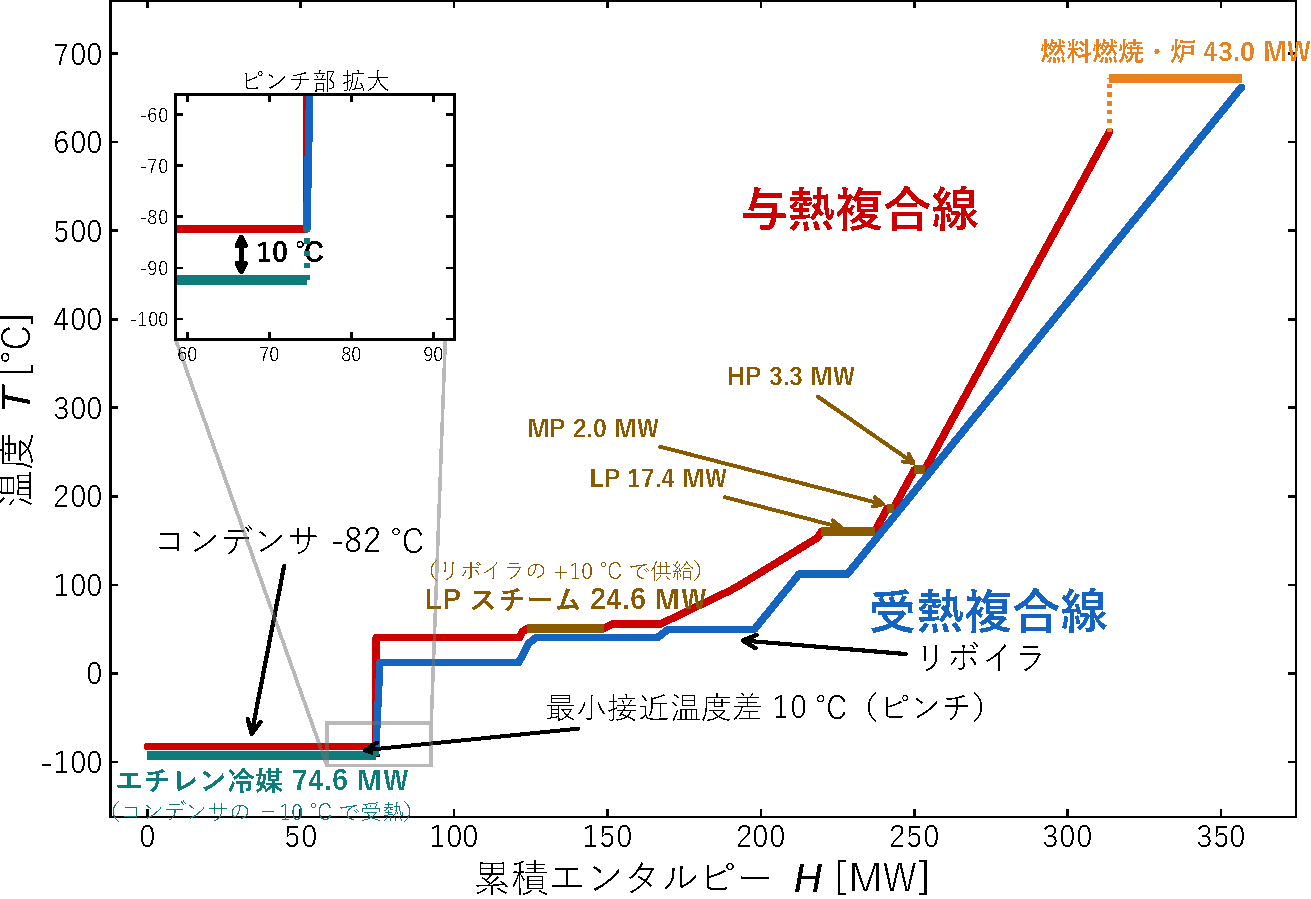
\includegraphics[width=\dimexpr\linewidth-2mm\relax]{composite_slide}
\end{frame}
}

\end{document}
